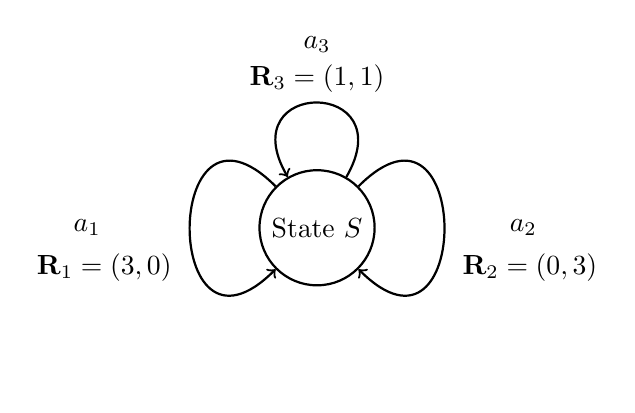
\begin{tikzpicture}
   \node[circle, thick, minimum size=1cm, draw=black] (state) {State \(S\)};
   \draw[thick, ->] (state) to [out=135, in=225, loop, looseness=5] node[left=10mm] {\(a_1\)} node [below=5mm, left=1mm] {\(\mathbf{R}_1 = (3, 0)\)} (state);
   \draw[thick, ->] (state) to [out=45, in=315, loop, looseness=5] node[right=7mm] {\(a_2\)} node [below=5mm, right=1mm] {\(\mathbf{R}_2 = (0, 3)\)} (state);
   \draw[thick, ->] (state) to [out=60, in=120, loop, looseness=5] node[above=5mm] {\(a_3\)} node [above=0mm] {\(\mathbf{R}_3 = (1, 1)\)} (state);
\end{tikzpicture}
